
\subsubsection{Polymorph}
Il design pattern \textit{Polymorph} è un pattern creato specificamente per le esigenze della codebase di Basalt. Esso 
è derivante dal pattern Type-Erasure, ma con alcune sostanziali differenze. \\

\begin{figure}[H]
    \centering
        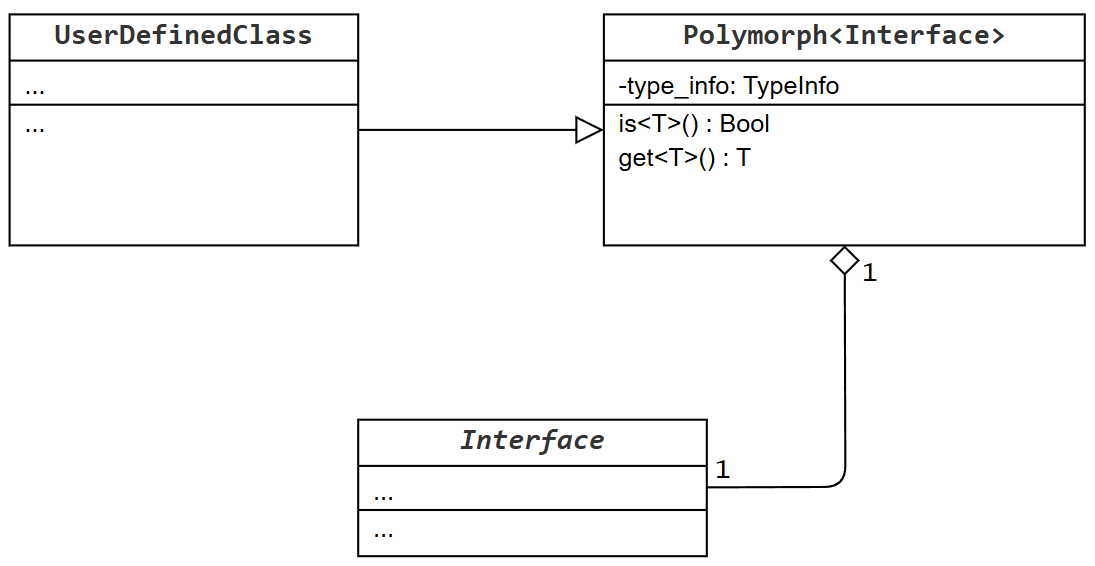
\includegraphics[width=0.7\textwidth]{../../Assets/Polymorph.png}
    \caption{UML class diagram del pattern Polymporph}
\end{figure}

Ogni classe definita dal client (ad esempio \texttt{UserDefinedClass}) deve estendere la classe \texttt{Polymorph<Interface>}. 
Facendo così, essa erediterà i metodi concreti \texttt{is} e \texttt{get} che permettono di fare \textit{downcasting}
dell'oggetto a runtime. \\

Contemporaneamente, sarà possibile assegnare a oggetti di tipo \texttt{UserDefinedClass} oggetti di tipo \texttt{T} purchè 
\texttt{T} estenda la classe \texttt{Interface} mediante ereditarietà. \\

Assegnando un oggetto di tipo \texttt{T} a un oggetto di tipo \texttt{UserDefinedClass} allora, essa utilizzerà l'operatore 
di assegnazione definito in \texttt{Polymorph} per assegnare ad un puntatore ad \texttt{Interface} l'oggetto che si desidera assegnare
ed aggiornare delle variabili interne per mantenere traccia del tipo dell'oggetto assegnato. \\

All'occorrenza si potrà interrogare la classe \texttt{UserDefinedClass} per sapere se contiene un oggetto di tipo \texttt{T}
o meno, utilizzando il metodo \texttt{is} e fare il \textit{downcasting} dell'oggetto a runtime utilizzando il metodo \texttt{get}. \\

\newpage

Di seguito è riportato un esempio di implementazione del pattern \textit{Polymorph}, così come è stato appena descritto,
al netto della classe \texttt{UserDefinedClass}: \\

\vspace{0.5cm}
\begin{lstlisting}[language=C++, frame=single]
class Interface {
    public:
        //...
};

template <typename Interface>
class Polymorph {
    private:
        std::shared_ptr<Concept> ptr = nullptr;
        TypeInfo type_info;

    public:
        template <typename Implementation>
        Polymorph& operator=(Implementation obj) {
            ptr = std::make_shared<Interface>(obj);
            type_info = TypeInfo::from<Implementation>();
        }

        template <typename Implementation>
        bool is<>() 
            requires(std::is_base_of_v<Interface, Implementation>)
        { 
            return TypeInfo::from<Implementation>() 
                == type_info; 
        }

        template <typename Implementation>
        Implementation& get() 
            requires(std::is_base_of_v<Interface, Implementation>)
        {
            if (is<Implementation>()) {
                return *static_cast<Implementation*>(ptr.get());
            }
            throw std::runtime_error("Invalid downcast");
        }
}
\end{lstlisting}
\vspace{0.5cm}

\texttt{Interface} in questo caso serve solo ad essere estesa da tutte e sole le classi che si desidera 
assegnare al \texttt{Polymorph}. L'estendere \texttt{Interface} è necessario in quanto è stato 
introdotto tale vincolo usando \texttt{requires(std::is\_base\_of\_v<T,U>)} (C++20 concepts).

\newpage

\subsubsection{Notazioni e diagrammistica}
Dato che questi design pattern servono a rendere il codice più leggibile e mantenibile, astraendo rispetto 
a come un certo comportamento polimorfico sia stato implementato, non renderebbe giustiza alla codebase di Basalt 
l'essere rappresentata con un UML class diagram tradizionale, in quanto essa risulterebbe artificiosamente più complessa. Per 
questo motivo, si è deciso di utilizzare la notazione UML di sotto-tipo (is-a relationship) per rappresentare
non solo l'ereditarietà, ma anche l'implementazione di questi design pattern i quali rispecchiano proprio una 
relazione di sotto-tipo. \\

\begin{figure}[H]
    \begin{tikzpicture}
        \node (before) at(-1, 0) {
            \resizebox{9cm}{6cm}{   
                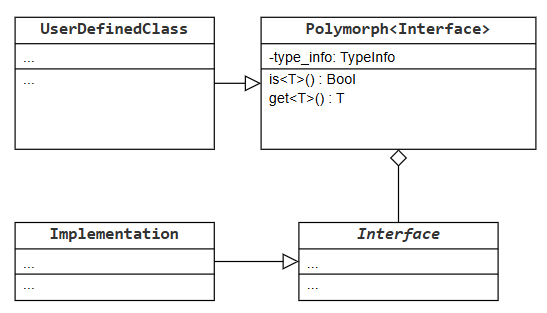
\includegraphics{../../Assets/Polymorph2.png}
            }
        };  

    
        \node[right of=before, xshift=7.5cm] (after) { 
            \resizebox{6cm}{8cm}{   
                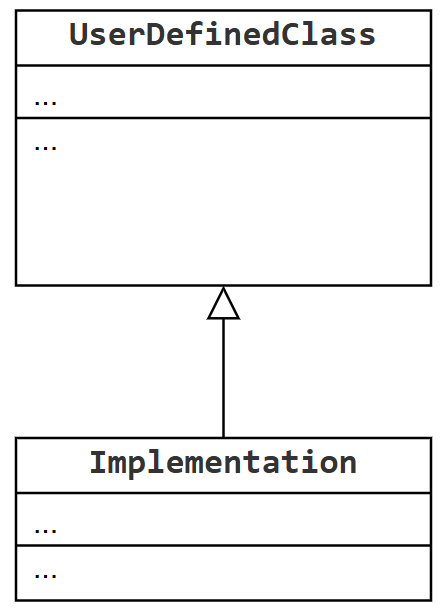
\includegraphics{../../Assets/Polymorph3.png}
            }
        };  

        \draw[->] (before) -- (after);
    \end{tikzpicture}
    \caption{
        \centering
        Traduzione UML del pattern Polymorph
    }
\end{figure}

\begin{figure}[H]
    \begin{tikzpicture}
        \node (before) {
            \resizebox{6.5cm}{6cm}{   
                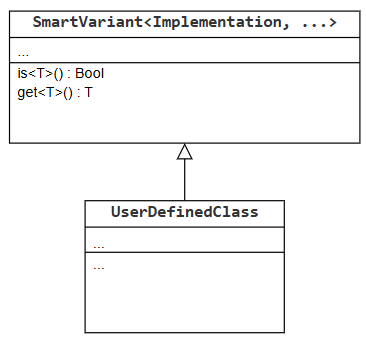
\includegraphics{../../Assets/SmartVariant.png}
            }
        };  

    
        \node[right of=before, xshift=7cm] (after) { 
            \resizebox{6cm}{8cm}{   
                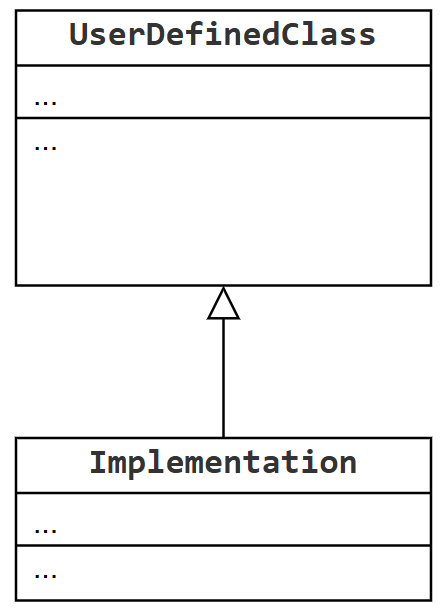
\includegraphics{../../Assets/Polymorph3.png}
            }
        };  

        \draw[->] (before) -- (after);
    \end{tikzpicture}
    \caption{
        \centering
        Traduzione UML del pattern Variant
    }
\end{figure}